\documentclass[sigconf]{acmart}
% 
% LaTeX template for visualizing the performance of
% optimization algorithms, that were run on the 
% bbob-noisy test suite of COCO. Any number of 
% algorithms should work with this template.
%

% include preamble:
%%%%%%%%%%%%%%%%%%%%%%%%%%%%%%%%%%%%%%%%%%%%%%%%%%%%%%%%%%%%%%%%%%%%%%%%%%%%%%%
% preamble for the BBOB ACM-compliant LaTeX templates                         %
%                                                                             %
% copyright 2009--2023 the BBOBies                                            %
% (under BSD licence, see https://github.com/numbbo/coco/blob/master/LICENSE) %
%%%%%%%%%%%%%%%%%%%%%%%%%%%%%%%%%%%%%%%%%%%%%%%%%%%%%%%%%%%%%%%%%%%%%%%%%%%%%%%

% to be updated from year to year:
\titlenote{Submission deadline: to be announced (likely late March/early April.}
\newcommand{\version}{2.6}


% Packages
\usepackage{booktabs} % For formal tables
\usepackage{graphicx}
\usepackage{rotating}
\usepackage{tabularx}
\usepackage{xspace}  % automatic white space after macros
\usepackage{xstring} % for string operations
\usepackage{wasysym} % Table legend with symbols input from post-processing
\usepackage{MnSymbol} % Table legend with symbols input from post-processing
\usepackage{float}
%\usepackage[dvipsnames]{xcolor}
%\usepackage[colorlinks=true, linkcolor=blue]{hyperref} % make COCO papers clickable
\usepackage{ifthen}
\usepackage{xcolor}



% define some COCO/dvipsnames colors because
% ACM style does not allow to use them directly
\definecolor{Gray}{gray}{0.6}
\definecolor{NavyBlue}{rgb}{0.0, 0.0, 0.5}
\definecolor{Magenta}{rgb}{1.0, 0.0, 1.0}
\definecolor{Black}{rgb}{0.0, 0.0, 0.0}
\definecolor{Green}{rgb}{0.0, 1.0, 0.0}
%\definecolor{NavyBlue}{HTML}{000080}
%\definecolor{Magenta}{HTML}{FF00FF}
%\definecolor{Orange}{HTML}{FFA500}
%\definecolor{CornflowerBlue}{HTML}{6495ED}
%\definecolor{YellowGreen}{HTML}{9ACD32}
%\definecolor{Gray}{HTML}{BEBEBE}
%\definecolor{Yellow}{HTML}{FFFF00}
%\definecolor{GreenYellow}{HTML}{ADFF2F}
%\definecolor{ForestGreen}{HTML}{228B22}
%\definecolor{Lavender}{HTML}{FFC0CB}
%\definecolor{SkyBlue}{HTML}{87CEEB}
%\definecolor{NavyBlue}{HTML}{000080}
%\definecolor{Goldenrod}{HTML}{DDF700}
%\definecolor{VioletRed}{HTML}{D02090}
%\definecolor{CornflowerBlue}{HTML}{6495ED}
%\definecolor{LimeGreen}{HTML}{32CD32}

% COCO LaTeX commands:
\newcommand{\includeperfprof}[1]{% include and annotate at the side
  \input{\bbobdatapath\algsfolder #1}%
  \includegraphics[height=0.24\textheight]{#1}%
  %\raisebox{.12\textheight}{
	%\parbox[b][.24\textheight]{.0868\textwidth}{\begin{scriptsize}
  %  \perfprofsidepanel % this is "\algaperfprof \vfill \algbperfprof \vfill" etc
  %\end{scriptsize}}
	%}
}
\newcommand{\rot}[2][2.5]{
  \hspace*{-3.5\baselineskip}%
  \begin{rotate}{90}\hspace{#1em}#2
  \end{rotate}}
\newcommand{\DIM}{\ensuremath{\mathrm{DIM}}}
\newcommand{\ERT}{\ensuremath{\mathrm{ERT}}}
\newcommand{\FEvals}{\ensuremath{\mathrm{FEvals}}}
\newcommand{\nruns}{\ensuremath{\mathrm{Nruns}}}
\newcommand{\Dfb}{\ensuremath{\Delta f_{\mathrm{best}}}}
\newcommand{\Df}{\ensuremath{\Delta f}}
\newcommand{\Dfg}{\ensuremath{\Delta \tau}}
\newcommand{\nbFEs}{\ensuremath{\mathrm{\#FEs}}}
\newcommand{\fopt}{\ensuremath{f_\mathrm{opt}}}
\newcommand{\ftarget}{\ensuremath{f_\mathrm{t}}}
\newcommand{\fgtarget}{\ensuremath{\tau_\mathrm{t}}}
\newcommand{\Itarget}{\ensuremath{I_\mathrm{target}}}
\newcommand{\CrE}{\ensuremath{\mathrm{CrE}}}
\newcommand{\change}[1]{{\color{red} #1}}
\newcommand{\TODO}[1]{{\color{orange} !!! #1 !!!}}
\newcommand{\bbob}{{\ttfamily bbob}\xspace}
\newcommand{\bbobnoisy}{{\ttfamily bbob-noisy}\xspace}
\newcommand{\bbobbiobj}{{\ttfamily bbob-biobj}\xspace}
\newcommand{\bbobls}{{\ttfamily bbob-largescale}\xspace}
\newcommand{\bbobmixint}{{\ttfamily bbob-mixint}\xspace}
\newcommand{\bbobcons}{{\ttfamily bbob-constrained}\xspace}
\newcommand{\DI}{\ensuremath{\Delta I_{\mathrm{HV}}^{\mathrm{COCO}}}}
\newcommand{\hvref}{\ensuremath{I_\mathrm{ref}}}


\usepackage{xcolor}
\usepackage{colortbl}
\usepackage{booktabs}
%It sets your colour line and then sets back to default (black)
\definecolor{bbobblue}{HTML}{7f7fff}
\definecolor{bbobgreen}{HTML}{7fbf7f}
\newcommand{\blueline}{\arrayrulecolor{bbobblue}\specialrule{0.15em}{0em}{0em}\arrayrulecolor{black}}
\newcommand{\greenline}{\arrayrulecolor{bbobgreen}\specialrule{0.15em}{0em}{0em}\arrayrulecolor{black}}


%%%%%%%%%%%%%%%%%%%%%%   END OF PREAMBLE   %%%%%%%%%%%%%%%%%%%%%%%%%%%%%%%%%%%%


% Copyright
%\setcopyright{none}
%\setcopyright{acmcopyright}
%\setcopyright{acmlicensed}
\setcopyright{rightsretained}
%\setcopyright{usgov}
%\setcopyright{usgovmixed}
%\setcopyright{cagov}
%\setcopyright{cagovmixed}


%%%%%%%%%%%%%%%%%%%%%%%%%%%%%%%%%%%%%%%%%%%%%%%%%%%%%


% DOI
\acmDOI{10.1145/nnnnnnn.nnnnnnn} % To be updated after completing copyright process

% ISBN
\acmISBN{978-x-xxxx-xxxx-x/YY/MM} % To be updated after completing copyright process

%Conference
\acmConference[GECCO '23]{The Genetic and Evolutionary Computation Conference 2023}{July 15--19, 2023}{Lisbon, Portugal}
\acmYear{2023}
\copyrightyear{2023}

\acmPrice{15.00}






%%%%%%%%%%%%%%%%%%%%%%   END OF PREAMBLE   %%%%%%%%%%%%%%%%%%%%%%%%%%%%%%%%%%%%



%%%%%%%%%%%%%%%%%%%%%%%%%%%%%%%%%%%%%%%%%%%%%%%%%%%%%%%%%%%%%%%%%%%%%%%%%%%%%%%
%%%%%%%%% TO BE EDITED %%%%%%%%%%%%%%%%%%%%%%%%%%%%%%%%%%%%%%%%%%%%%%%%%%%%%%%%
%%%%%%%%%%%%%%%%%%%%%%%%%%%%%%%%%%%%%%%%%%%%%%%%%%%%%%%%%%%%%%%%%%%%%%%%%%%%%%%

% Algorithm names as they appear in the tables, uncomment and adapt if necessary
% \newcommand{\algAtables}{ALGO1}  % first argument in the post-processing
% \newcommand{\algBtables}{ALGO2}  % second argument in the post-processing
% \newcommand{\algCtables}{ALGO3}  % third argument in the post-processing
% \newcommand{\algDtables}{ALGO4}  % forth argument in the post-processing
% ...
% location of pictures files
\newcommand{\bbobdatapath}{ppdata/} % change default output folder of COCO if desired



%%%%%%%%%%%%%%%%%%%%%%%%%%%%%%%%%%%%%%%%%%%%%%%%%%%%%%%%%%%%%%%%%%%%%%%%%%%%%%%
% read in data and deal with the different number of algorithms:
\input{\bbobdatapath cocopp_commands.tex}
\ifthenelse{\equal{\numofalgs}{1}}
{
    \newcommand{\numberofalgorithms}{one}
}
{
    \ifthenelse{\equal{\numofalgs}{2}}
    {
        \newcommand{\numberofalgorithms}{two}
    }{
	    \newcommand{\numberofalgorithms}{three}
	}
}


\ifthenelse{\equal{\numberofalgorithms}{one}}{
   \graphicspath{{\bbobdatapath\algfolder}}}{
	 \graphicspath{{\bbobdatapath\algsfolder}}
}

\ifthenelse{\isundefined{\algorithmA}}{\newcommand{\algorithmA}{\algname}}{}
%\ifthenelse{\isundefined{\algorithmA}{\newcommand{\algorithmA}{\change{MY-ALGORITHM-NAME}}}{}  % better use the previous line?
%%



%%%%%%%%%%%%%%%%%%%%%%%%%%%%%%%%%%%%%%%%%%%%%%%%%%%%%%%%%%%%%%%%%%%%%%%%%%%%%%%
%%%%%%%%%%%%%%%%%%%%%%%%%%%%%%%%%%%%%%%%%%%%%%%%%%%%%%%%%%%%%%%%%%%%%%%%%%%%%%%
%%%%%%%%%%%%%%%%%%%%%%%%%%%%%%%%%%%%%%%%%%%%%%%%%%%%%%%%%%%%%%%%%%%%%%%%%%%%%%%

\begin{document}


\title{Black-Box Optimization Benchmarking Template for the Comparison of Algorithms on the \bbobnoisy Testbed}
\renewcommand{\shorttitle}{Template to Compare Algorithms on the \bbobnoisy Testbed}
\subtitle{Draft version}



\author{Firstname Lastname}
%\authornote{tba if needed}
%\orcid{1234-5678-9012}
%\affiliation{%
%  \institution{Institute for Clarity in Documentation}
%  \streetaddress{P.O. Box 1212}
%  \city{Dublin} 
%  \state{Ohio} 
%  \postcode{43017-6221}
%}
%\email{trovato@corporation.com}
%
%\author{G.K.M. Tobin}
%\authornote{The secretary disavows any knowledge of this author's actions.}
%\affiliation{%
%  \institution{Institute for Clarity in Documentation}
%  \streetaddress{P.O. Box 1212}
%  \city{Dublin} 
%  \state{Ohio} 
%  \postcode{43017-6221}
%}
%\email{webmaster@marysville-ohio.com}
%
%\author{Lars Th{\o}rv{\"a}ld}
%\authornote{This author is the
%  one who did all the really hard work.}
%\affiliation{%
%  \institution{The Th{\o}rv{\"a}ld Group}
%  \streetaddress{1 Th{\o}rv{\"a}ld Circle}
%  \city{Hekla} 
%  \country{Iceland}}
%\email{larst@affiliation.org}
%
%\author{Lawrence P. Leipuner}
%\affiliation{
%  \institution{Brookhaven Laboratories}
%  \streetaddress{P.O. Box 5000}}
%\email{lleipuner@researchlabs.org}
%
%\author{Sean Fogarty}
%\affiliation{%
%  \institution{NASA Ames Research Center}
%  \city{Moffett Field}
%  \state{California} 
%  \postcode{94035}}
%\email{fogartys@amesres.org}
%
%\author{Charles Palmer}
%\affiliation{%
%  \institution{Palmer Research Laboratories}
%  \streetaddress{8600 Datapoint Drive}
%  \city{San Antonio}
%  \state{Texas} 
%  \postcode{78229}}
%\email{cpalmer@prl.com}
%
%\author{John Smith}
%\affiliation{\institution{The Th{\o}rv{\"a}ld Group}}
%\email{jsmith@affiliation.org}
%
%\author{Julius P.~Kumquat}
%\affiliation{\institution{The Kumquat Consortium}}
%\email{jpkumquat@consortium.net}

% The default list of authors is too long for headers}
\renewcommand{\shortauthors}{Firstname Lastname et. al.}


\begin{abstract}
to be written
\end{abstract}


%
% The code below should be generated by the tool at
% http://dl.acm.org/ccs.cfm
% Please copy and paste the code instead of the example below. 
%
 \begin{CCSXML}
<ccs2012>
<concept>
<concept_id>10010147.10010178.10010205.10010208</concept_id>
<concept_desc>Computing methodologies~Continuous space search</concept_desc>
<concept_significance>500</concept_significance>
</concept>
</ccs2012>
\end{CCSXML}

\ccsdesc[500]{Computing methodologies~Continuous space search}


% We no longer use \terms command
%\terms{Algorithms}

% Complete with anything that is needed
\keywords{Benchmarking, Black-box optimization, Noisy optimization}

\maketitle


% \section{Introduction}
%
% \section{Algorithm Presentation}
%
% \section{Experimental Procedure}
%

%%%%%%%%%%%%%%%%%%%%%%%%%%%%%%%%%%%%%%%%%%%%%%%%%%%%%%%%%%%%%%%%%%%%%%%%%%%%%%%
\section{CPU Timing}
%%%%%%%%%%%%%%%%%%%%%%%%%%%%%%%%%%%%%%%%%%%%%%%%%%%%%%%%%%%%%%%%%%%%%%%%%%%%%%%
% note that the following text is just a proposal and can/should be changed to your needs:
In order to evaluate the CPU timing of the algorithm, we have run the \change{\algorithmA} with restarts on the entire \bbobnoisy test suite \cite{hansen2010noi} for \change{$2 D$} function evaluations according to \cite{hansen2016exp}.
\change{replace the previous sentence with ``on the function $f_{8}$ with restarts for at least 30 seconds and until a maximum budget equal to \change{$400 (D + 2)$} is reached.'' in case you use the old code base}
 The \change{C/Java/Matlab/Octave/Python} code was run on a \change{Mac Intel(R) Core(TM) i5-2400S CPU @ 2.50GHz} with \change{1} processor and \change{4} cores \change{and (compile) options xxx}. The time per function evaluation for dimensions 2, 3, 5, 10, 20\change{, 40} equals \change{$x.x$}, \change{$x.x$}, \change{$x.x$}, \change{$xx$}, \change{$xxx$}\change{, and $xxx$} seconds respectively. 

\ifthenelse{\equal{\numberofalgorithms}{one}}{}{
\change{repeat the above for any algorithm tested}
}

%%%%%%%%%%%%%%%%%%%%%%%%%%%%%%%%%%%%%%%%%%%%%%%%%%%%%%%%%%%%%%%%%%%%%%%%%%%%%%%
\section{Results}
%%%%%%%%%%%%%%%%%%%%%%%%%%%%%%%%%%%%%%%%%%%%%%%%%%%%%%%%%%%%%%%%%%%%%%%%%%%%%%%

Results from experiments according to \cite{hansen2016exp} and
\cite{hansen2022anytime} on the benchmark functions given in 
\cite{hansen2010noi} are presented in
%%
\ifthenelse{\equal{\numberofalgorithms}{one}}{
Figures~\ref{fig:ERTgraphs}, \ref{fig:ECDFs}, and \ref{fig:ECDFsingleOne} and Tables~\ref{tab:ERTs}, \ref{tab:ERTloss}, and \ref{fig:ERTlogloss}.
}{\ifthenelse{\equal{\numberofalgorithms}{two}}{
Figures~\ref{fig:scaling}, \ref{fig:ECDFs}, \ref{fig:ECDFsingleOne}, and \ref{fig:scatterplots} and Tables~\ref{tab:ERTs5} and \ref{tab:ERTs20}.
}{\ifthenelse{\equal{\numberofalgorithms}{three}}{
Figures~\ref{fig:scaling}, \ref{fig:ECDFs}, and \ref{fig:ECDFsingleOne} and Tables~\ref{tab:ERTs5} and \ref{tab:ERTs20}.
}{}}}
%%
The experiments were performed with COCO \cite{hansen2020cocoplat}, version
\change{\version}, the plots were produced with version \change{\version}.

The \textbf{expected runtime (ERT)}, used in the %figures and
tables,
depends on a given target precision, $\Itarget=\fopt+\Df$, and is
computed over all relevant trials as the number of function
evaluations executed during each trial while the best function value
did not reach \ftarget, summed over all trials and divided by the
number of trials that actually reached \ftarget\
\cite{hansen2016exp,price1997dev}.
\textbf{Statistical significance} is tested with the rank-sum test for a given
target $\Delta\ftarget$ using, for each trial,
either the number of needed function evaluations to reach
$\ftarget$ (inverted and multiplied by $-1$), or, if the target
was not reached, the best $\Df$-value achieved, measured only up to
the smallest number of overall function evaluations for any
unsuccessful trial under consideration.



\ifthenelse{\equal{\numberofalgorithms}{one}}{

%%%%%%%%%%%%%%%%%%%%%%%%%%%%%%%%%%%%%%%%%%%%%%%%%%%%%%%%%%%%%%%%%%%%%%%%%%%%%%%

% Scaling of ERT with dimension 

%%%%%%%%%%%%%%%%%%%%%%%%%%%%%%%%%%%%%%%%%%%%%%%%%%%%%%%%%%%%%%%%%%%%%%%%%%%%%%
\begin{figure*}
\centering
\begin{tabular}{l@{\hspace*{-0.001\textwidth}}l@{\hspace*{-0.001\textwidth}}l@{\hspace*{-0.001\textwidth}}l@{\hspace*{-0.001\textwidth}}l}
\includegraphics[width=0.2\textwidth,]{ppfigdim_f101}&
\includegraphics[width=0.2\textwidth]{ppfigdim_f104}&
\includegraphics[width=0.2\textwidth]{ppfigdim_f107}&
\includegraphics[width=0.2\textwidth]{ppfigdim_f110}&
\includegraphics[width=0.2\textwidth]{ppfigdim_f113}\\
\includegraphics[width=0.2\textwidth]{ppfigdim_f102}&
\includegraphics[width=0.2\textwidth]{ppfigdim_f105}&
\includegraphics[width=0.2\textwidth]{ppfigdim_f108}&
\includegraphics[width=0.2\textwidth]{ppfigdim_f111}&
\includegraphics[width=0.2\textwidth]{ppfigdim_f114}\\
\includegraphics[width=0.2\textwidth]{ppfigdim_f103}&
\includegraphics[width=0.2\textwidth]{ppfigdim_f106}&
\includegraphics[width=0.2\textwidth]{ppfigdim_f109}&
\includegraphics[width=0.2\textwidth]{ppfigdim_f112}&
\includegraphics[width=0.2\textwidth]{ppfigdim_f115}\\\hline
\includegraphics[width=0.2\textwidth]{ppfigdim_f116}&
\includegraphics[width=0.2\textwidth]{ppfigdim_f119}&
\includegraphics[width=0.2\textwidth]{ppfigdim_f122}&
\includegraphics[width=0.2\textwidth]{ppfigdim_f125}&
\includegraphics[width=0.2\textwidth]{ppfigdim_f128}\\
\includegraphics[width=0.2\textwidth]{ppfigdim_f117}&
\includegraphics[width=0.2\textwidth]{ppfigdim_f120}&
\includegraphics[width=0.2\textwidth]{ppfigdim_f123}&
\includegraphics[width=0.2\textwidth]{ppfigdim_f126}&
\includegraphics[width=0.2\textwidth]{ppfigdim_f129}\\
\includegraphics[width=0.2\textwidth]{ppfigdim_f118}&
\includegraphics[width=0.2\textwidth]{ppfigdim_f121}&
\includegraphics[width=0.2\textwidth]{ppfigdim_f124}&
\includegraphics[width=0.2\textwidth]{ppfigdim_f127}&
\includegraphics[width=0.2\textwidth]{ppfigdim_f130}\\
\end{tabular}
\vspace{-1ex}
 \caption{
 \label{fig:ERTgraphs}
 \bbobppfigdimlegend{$f_{101}$ and $f_{130}$}
 }
\end{figure*}


%%%%%%%%%%%%%%%%%%%%%%%%%%%%%%%%%%%%%%%%%%%%%%%%%%%%%%%%%%%%%%%%%%%%%%%%%%%%%%%
%%%%%%%%%%%%%%%%%%%%%%%%%%%%%%%%%%%%%%%%%%%%%%%%%%%%%%%%%%%%%%%%%%%%%%%%%%%%%%%

% Empirical Cumulative Distribution Functions (ECDFs) per function group
% in all dimensions.

%%%%%%%%%%%%%%%%%%%%%%%%%%%%%%%%%%%%%%%%%%%%%%%%%%%%%%%%%%%%%%%%%%%%%%%%%%%%%%%
\begin{figure*}
	\centering
	\begin{tabular}{@{}c@{}c@{}}
		{\Large\sffamily moderate noise} & {\Large\sffamily severe noise}\\
		\includegraphics[width=0.49\textwidth]{pprldmany-single-functions/pprldmany_nzmod} & 
		\includegraphics[width=0.49\textwidth]{pprldmany-single-functions/pprldmany_nzsev}\\[0.5em]
		{\Large\sffamily severe noise multimod.} & {\Large\sffamily all functions}\\
		\includegraphics[width=0.49\textwidth]{pprldmany-single-functions/pprldmany_nzsmm} &
		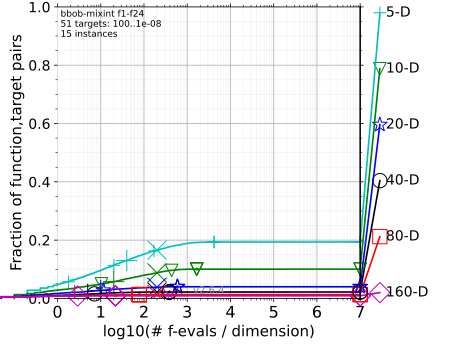
\includegraphics[width=0.49\textwidth]{pprldmany-single-functions/pprldmany}\\[-0.5em]
	\end{tabular}
\caption{\label{fig:ECDFs} \bbobecdfcaptionallgroups}
\end{figure*}


%%%%%%%%%%%%%%%%%%%%%%%%%%%%%%%%%%%%%%%%%%%%%%%%%%%%%%%%%%%%%%%%%%%%%%%%%%%%%%%
%%%%%%%%%%%%%%%%%%%%%%%%%%%%%%%%%%%%%%%%%%%%%%%%%%%%%%%%%%%%%%%%%%%%%%%%%%%%%%%

% ECDFs per function

%%%%%%%%%%%%%%%%%%%%%%%%%%%%%%%%%%%%%%%%%%%%%%%%%%%%%%%%%%%%%%%%%%%%%%%%%%%%%%%
\begin{figure*}
\centering
\begin{tabular}{l@{\hspace*{-0.01\textwidth}}l@{\hspace*{-0.01\textwidth}}l@{\hspace*{-0.01\textwidth}}l@{\hspace*{-0.01\textwidth}}l@{\hspace*{-0.01\textwidth}}}
\includegraphics[width=0.21\textwidth]{pprldmany-single-functions/pprldmany_f101}&
\includegraphics[width=0.21\textwidth]{pprldmany-single-functions/pprldmany_f104}&
\includegraphics[width=0.21\textwidth]{pprldmany-single-functions/pprldmany_f107}&
\includegraphics[width=0.21\textwidth]{pprldmany-single-functions/pprldmany_f110}&
\includegraphics[width=0.21\textwidth]{pprldmany-single-functions/pprldmany_f113}\\
\includegraphics[width=0.21\textwidth]{pprldmany-single-functions/pprldmany_f102}&
\includegraphics[width=0.21\textwidth]{pprldmany-single-functions/pprldmany_f105}&
\includegraphics[width=0.21\textwidth]{pprldmany-single-functions/pprldmany_f108}&
\includegraphics[width=0.21\textwidth]{pprldmany-single-functions/pprldmany_f111}&
\includegraphics[width=0.21\textwidth]{pprldmany-single-functions/pprldmany_f114}\\
\includegraphics[width=0.21\textwidth]{pprldmany-single-functions/pprldmany_f103}&
\includegraphics[width=0.21\textwidth]{pprldmany-single-functions/pprldmany_f106}&
\includegraphics[width=0.21\textwidth]{pprldmany-single-functions/pprldmany_f109}&
\includegraphics[width=0.21\textwidth]{pprldmany-single-functions/pprldmany_f112}&
\includegraphics[width=0.21\textwidth]{pprldmany-single-functions/pprldmany_f115}\\\hline\\
\includegraphics[width=0.21\textwidth]{pprldmany-single-functions/pprldmany_f116}&
\includegraphics[width=0.21\textwidth]{pprldmany-single-functions/pprldmany_f119}&
\includegraphics[width=0.21\textwidth]{pprldmany-single-functions/pprldmany_f122}&
\includegraphics[width=0.21\textwidth]{pprldmany-single-functions/pprldmany_f125}&
\includegraphics[width=0.21\textwidth]{pprldmany-single-functions/pprldmany_f128}\\
\includegraphics[width=0.21\textwidth]{pprldmany-single-functions/pprldmany_f117}&
\includegraphics[width=0.21\textwidth]{pprldmany-single-functions/pprldmany_f120}&
\includegraphics[width=0.21\textwidth]{pprldmany-single-functions/pprldmany_f123}&
\includegraphics[width=0.21\textwidth]{pprldmany-single-functions/pprldmany_f126}&
\includegraphics[width=0.21\textwidth]{pprldmany-single-functions/pprldmany_f129}\\
\includegraphics[width=0.21\textwidth]{pprldmany-single-functions/pprldmany_f118}&
\includegraphics[width=0.21\textwidth]{pprldmany-single-functions/pprldmany_f121}&
\includegraphics[width=0.21\textwidth]{pprldmany-single-functions/pprldmany_f124}&
\includegraphics[width=0.21\textwidth]{pprldmany-single-functions/pprldmany_f127}&
\includegraphics[width=0.21\textwidth]{pprldmany-single-functions/pprldmany_f130}\\[-1.0ex]
\end{tabular}
 \caption{\label{fig:ECDFsingleOne}
	\bbobecdfcaptionsinglefunctionssingledim{$\!\!$s 2 to 40}
}
\end{figure*}


%%%%%%%%%%%%%%%%%%%%%%%%%%%%%%%%%%%%%%%%%%%%%%%%%%%%%%%%%%%%%%%%%%%%%%%%%%%%%%%

% Table showing the expected running time (ERT in number of function
% evaluations) divided by the the ERT of a reference algorithm (e.g. the best
% measured ERT during BBOB-2009) as given in the first row of each cell
% for functions $f_101$--$f_{130}$.

%%%%%%%%%%%%%%%%%%%%%%%%%%%%%%%%%%%%%%%%%%%%%%%%%%%%%%%%%%%%%%%%%%%%%%%%%%%%%%%
\begin{table*}
\centering 
\mbox{\begin{minipage}[t]{0.499\textwidth}
\centering
5-D\\
\tiny
\pptableheader 
\input{\bbobdatapath\algfolder pptable_f101_05D} 
\input{\bbobdatapath\algfolder pptable_f102_05D}
\input{\bbobdatapath\algfolder pptable_f103_05D}
\input{\bbobdatapath\algfolder pptable_f104_05D}
\input{\bbobdatapath\algfolder pptable_f105_05D}
\input{\bbobdatapath\algfolder pptable_f106_05D}
\input{\bbobdatapath\algfolder pptable_f107_05D}
\input{\bbobdatapath\algfolder pptable_f108_05D}
\input{\bbobdatapath\algfolder pptable_f109_05D}
\input{\bbobdatapath\algfolder pptable_f110_05D}
\input{\bbobdatapath\algfolder pptable_f111_05D}
\input{\bbobdatapath\algfolder pptable_f112_05D}
\input{\bbobdatapath\algfolder pptable_f113_05D}
\input{\bbobdatapath\algfolder pptable_f114_05D}
\input{\bbobdatapath\algfolder pptable_f115_05D}
\input{\bbobdatapath\algfolder pptable_f116_05D}
\input{\bbobdatapath\algfolder pptable_f117_05D}
\input{\bbobdatapath\algfolder pptable_f118_05D}
\input{\bbobdatapath\algfolder pptable_f119_05D}
\input{\bbobdatapath\algfolder pptable_f120_05D}
\input{\bbobdatapath\algfolder pptable_f121_05D}
\input{\bbobdatapath\algfolder pptable_f122_05D}
\input{\bbobdatapath\algfolder pptable_f123_05D}
\input{\bbobdatapath\algfolder pptable_f124_05D}
\input{\bbobdatapath\algfolder pptable_f125_05D}
\input{\bbobdatapath\algfolder pptable_f126_05D}
\input{\bbobdatapath\algfolder pptable_f127_05D}
\input{\bbobdatapath\algfolder pptable_f128_05D}
\input{\bbobdatapath\algfolder pptable_f129_05D}
\input{\bbobdatapath\algfolder pptable_f130_05D}

\pptablefooter
\end{minipage}

\hspace{0.002\textwidth}

\begin{minipage}[t]{0.499\textwidth}
\centering
20-D\\
\tiny
\pptableheader 
\input{\bbobdatapath\algfolder pptable_f101_20D} 
\input{\bbobdatapath\algfolder pptable_f102_20D}
\input{\bbobdatapath\algfolder pptable_f103_20D}
\input{\bbobdatapath\algfolder pptable_f104_20D}
\input{\bbobdatapath\algfolder pptable_f105_20D}
\input{\bbobdatapath\algfolder pptable_f106_20D}
\input{\bbobdatapath\algfolder pptable_f107_20D}
\input{\bbobdatapath\algfolder pptable_f108_20D}
\input{\bbobdatapath\algfolder pptable_f109_20D}
\input{\bbobdatapath\algfolder pptable_f110_20D}
\input{\bbobdatapath\algfolder pptable_f111_20D}
\input{\bbobdatapath\algfolder pptable_f112_20D}
\input{\bbobdatapath\algfolder pptable_f113_20D}
\input{\bbobdatapath\algfolder pptable_f114_20D}
\input{\bbobdatapath\algfolder pptable_f115_20D}
\input{\bbobdatapath\algfolder pptable_f116_20D}
\input{\bbobdatapath\algfolder pptable_f117_20D}
\input{\bbobdatapath\algfolder pptable_f118_20D}
\input{\bbobdatapath\algfolder pptable_f119_20D}
\input{\bbobdatapath\algfolder pptable_f120_20D}
\input{\bbobdatapath\algfolder pptable_f121_20D}
\input{\bbobdatapath\algfolder pptable_f122_20D}
\input{\bbobdatapath\algfolder pptable_f123_20D}
\input{\bbobdatapath\algfolder pptable_f124_20D}
\input{\bbobdatapath\algfolder pptable_f125_20D}
\input{\bbobdatapath\algfolder pptable_f126_20D}
\input{\bbobdatapath\algfolder pptable_f127_20D}
\input{\bbobdatapath\algfolder pptable_f128_20D}
\input{\bbobdatapath\algfolder pptable_f129_20D}
\input{\bbobdatapath\algfolder pptable_f130_20D}\pptablefooter
\end{minipage}}
\vspace{1em}

\caption[Table of ERTs]{\label{tab:ERTs}
\bbobpptablecaption{dimensions $5$ (left) and $20$ (right)} \cocoversion
}
\end{table*}


%%%%%%%%%%%%%%%%%%%%%%%%%%%%%%%%%%%%%%%%%%%%%%%%%%%%%%%%%%%%%%%%%%%%%%%%%%%%%%%
%%%%%%%%%%%%%%%%%%%%%%%%%%%%%%%%%%%%%%%%%%%%%%%%%%%%%%%%%%%%%%%%%%%%%%%%%%%%%%%

% ERT loss ratios (figure and table)

%%%%%%%%%%%%%%%%%%%%%%%%%%%%%%%%%%%%%%%%%%%%%%%%%%%%%%%%%%%%%%%%%%%%%%%%%%%%%%%
\begin{figure}
\centering
\parbox{0.49\columnwidth}{\centering 5-D}%
\parbox{0.49\columnwidth}{\centering 20-D}\\
\includegraphics[width=0.24\textwidth]{pplogloss_05D_nzall}%
\includegraphics[width=0.24\textwidth]{pplogloss_20D_nzall}
%
\input{\bbobdatapath\algfolder pploglosstable_05D_nzall}\\
\input{\bbobdatapath\algfolder pploglosstable_20D_nzall}
\caption{\label{tab:ERTloss}%
\bbobloglosstablecaption{} \cocoversion
}
\end{figure}



%%%%%%%%%%%%%%%%%%%%%%%%%%%%%%%%%%%%%%%%%%%%%%%%%%%%%%%%%%%%%%%%%%%%%%%%%%%%%%%
%%%%%%%%%%%%%%%%%%%%%%%%%%%%%%%%%%%%%%%%%%%%%%%%%%%%%%%%%%%%%%%%%%%%%%%%%%%%%%%

% ERT loss ratios per function group

%%%%%%%%%%%%%%%%%%%%%%%%%%%%%%%%%%%%%%%%%%%%%%%%%%%%%%%%%%%%%%%%%%%%%%%%%%%%%%%
\begin{figure}
\begin{tabular}{@{}l@{}@{}l@{}}
\multicolumn{1}{c}{5-D} & \multicolumn{1}{c}{20-D}\\
\rot{moderate noise}
\hspace*{-1mm}
\includegraphics[width=0.24\textwidth]{pplogloss_05D_nzmod} &
\includegraphics[width=0.24\textwidth]{pplogloss_20D_nzmod} \\
\rot{$\,\,$severe noise}
\hspace*{-1mm}
\includegraphics[width=0.24\textwidth]{pplogloss_05D_nzsev} &
\includegraphics[width=0.24\textwidth]{pplogloss_20D_nzsev} \\
\rot[0.5]{severe noise multimod.}
\hspace*{-1mm}
\includegraphics[width=0.24\textwidth]{pplogloss_05D_nzsmm} &
\includegraphics[width=0.24\textwidth]{pplogloss_20D_nzsmm}
\end{tabular}
\caption{\label{fig:ERTlogloss}%
\bbobloglossfigurecaption{}
}
\end{figure}


%%%%%%%%%%%%%%%%%%%%%%%%%%%%%%%%%%%%%%%%%%%%%%%%%%%%%%%%%%%%%%%%%%%%%%%%%%%%%%%

}{} % end of 1 algorithm template




\ifthenelse{\equal{\numberofalgorithms}{two} \or \equal{\numberofalgorithms}{three}}{

%%%%%%%%%%%%%%%%%%%%%%%%%%%%%%%%%%%%%%%%%%%%%%%%%%%%%%%%%%%%%%%%%%%%%%%%%%%%%%%

% Scaling of ERT with dimension

%%%%%%%%%%%%%%%%%%%%%%%%%%%%%%%%%%%%%%%%%%%%%%%%%%%%%%%%%%%%%%%%%%%%%%%%%%%%%%%

\begin{figure*}
\centering
\begin{tabular}{@{}c@{}c@{}c@{}c@{}c@{}}
\includegraphics[width=0.2\textwidth]{ppfigs_f101}&
\includegraphics[width=0.2\textwidth]{ppfigs_f104}&
\includegraphics[width=0.2\textwidth]{ppfigs_f107}&
\includegraphics[width=0.2\textwidth]{ppfigs_f110}&
\includegraphics[width=0.2\textwidth]{ppfigs_f113}\\
\includegraphics[width=0.2\textwidth]{ppfigs_f102}&
\includegraphics[width=0.2\textwidth]{ppfigs_f105}&
\includegraphics[width=0.2\textwidth]{ppfigs_f108}&
\includegraphics[width=0.2\textwidth]{ppfigs_f111}&
\includegraphics[width=0.2\textwidth]{ppfigs_f114}\\
\includegraphics[width=0.2\textwidth]{ppfigs_f103}&
\includegraphics[width=0.2\textwidth]{ppfigs_f106}&
\includegraphics[width=0.2\textwidth]{ppfigs_f109}&
\includegraphics[width=0.2\textwidth]{ppfigs_f112}&
\includegraphics[width=0.2\textwidth]{ppfigs_f115}\\
\includegraphics[width=0.2\textwidth]{ppfigs_f116}&
\includegraphics[width=0.2\textwidth]{ppfigs_f119}&
\includegraphics[width=0.2\textwidth]{ppfigs_f122}&
\includegraphics[width=0.2\textwidth]{ppfigs_f125}&
\includegraphics[width=0.2\textwidth]{ppfigs_f128}\\
\includegraphics[width=0.2\textwidth]{ppfigs_f117}&
\includegraphics[width=0.2\textwidth]{ppfigs_f120}&
\includegraphics[width=0.2\textwidth]{ppfigs_f123}&
\includegraphics[width=0.2\textwidth]{ppfigs_f126}&
\includegraphics[width=0.2\textwidth]{ppfigs_f129}\\
\includegraphics[width=0.2\textwidth]{ppfigs_f118}&
\includegraphics[width=0.2\textwidth]{ppfigs_f121}&
\includegraphics[width=0.2\textwidth]{ppfigs_f124}&
\includegraphics[width=0.2\textwidth]{ppfigs_f127}&
\includegraphics[width=0.2\textwidth]{ppfigs_f130}
\end{tabular}
\caption[Expected running time (\ERT) divided by dimension
versus dimension in log-log presentation]{\label{fig:scaling}%
\bbobppfigslegend{$f_{101}$ and $f_{130}$}
}
\end{figure*}


%%%%%%%%%%%%%%%%%%%%%%%%%%%%%%%%%%%%%%%%%%%%%%%%%%%%%%%%%%%%%%%%%%%%%%%%%%%%%%%
%%%%%%%%%%%%%%%%%%%%%%%%%%%%%%%%%%%%%%%%%%%%%%%%%%%%%%%%%%%%%%%%%%%%%%%%%%%%%%%

% Empirical Cumulative Distribution Functions (ECDFs) per function group
% in dimensions 5 and 20.

%%%%%%%%%%%%%%%%%%%%%%%%%%%%%%%%%%%%%%%%%%%%%%%%%%%%%%%%%%%%%%%%%%%%%%%%%%%%%%%
\begin{figure*}
   \begin{tabular}{@{}c@{}c@{}c@{}}
      \,\, & 5-D & 20-D\\
			\rot{\Large\sffamily \,\,\,\,\,\,\,\,\,\,all functions}\hspace{1em} &
			   \includegraphics[height=0.25\textwidth]{pprldmany_05D_nzall} &
			   \includegraphics[height=0.25\textwidth]{pprldmany_20D_nzall}\\[1em]
			\rot{\Large\sffamily \,\,\,\,\,moderate noise}\hspace{1em} &
			   \includegraphics[height=0.25\textwidth]{pprldmany_05D_nzmod} &
			   \includegraphics[height=0.25\textwidth]{pprldmany_20D_nzmod}\\[1em]
			\rot{\Large\sffamily \,\,\,\,\,\,\,\,\,\,\,severe noise}\hspace{1em} &
			   \includegraphics[height=0.25\textwidth]{pprldmany_05D_nzsev} &
			   \includegraphics[height=0.25\textwidth]{pprldmany_20D_nzsev}\\[1em]
			\rot{\Large\sffamily \!\!severe noise multimod.}\hspace{1em} &
			   \includegraphics[height=0.25\textwidth]{pprldmany_05D_nzsmm} &
			   \includegraphics[height=0.25\textwidth]{pprldmany_20D_nzsmm}
    \end{tabular}
\caption{\label{fig:ECDFs} \bbobECDFslegend{$5$- and $20$}}
\end{figure*}


%%%%%%%%%%%%%%%%%%%%%%%%%%%%%%%%%%%%%%%%%%%%%%%%%%%%%%%%%%%%%%%%%%%%%%%%%%%%%%%
%%%%%%%%%%%%%%%%%%%%%%%%%%%%%%%%%%%%%%%%%%%%%%%%%%%%%%%%%%%%%%%%%%%%%%%%%%%%%%%

% ECDFs per function in dimension 10

%%%%%%%%%%%%%%%%%%%%%%%%%%%%%%%%%%%%%%%%%%%%%%%%%%%%%%%%%%%%%%%%%%%%%%%%%%%%%%%
\begin{figure*}
\centering
\begin{tabular}{@{}l@{}l@{}l@{}l@{}l@{}}
\includegraphics[width=0.2\textwidth]{pprldmany-single-functions/pprldmany_f101_10D}&
\includegraphics[width=0.2\textwidth]{pprldmany-single-functions/pprldmany_f104_10D}&
\includegraphics[width=0.2\textwidth]{pprldmany-single-functions/pprldmany_f107_10D}&
\includegraphics[width=0.2\textwidth]{pprldmany-single-functions/pprldmany_f110_10D}&
\includegraphics[width=0.2\textwidth]{pprldmany-single-functions/pprldmany_f113_10D}\\
\includegraphics[width=0.2\textwidth]{pprldmany-single-functions/pprldmany_f102_10D}&
\includegraphics[width=0.2\textwidth]{pprldmany-single-functions/pprldmany_f105_10D}&
\includegraphics[width=0.2\textwidth]{pprldmany-single-functions/pprldmany_f108_10D}&
\includegraphics[width=0.2\textwidth]{pprldmany-single-functions/pprldmany_f111_10D}&
\includegraphics[width=0.2\textwidth]{pprldmany-single-functions/pprldmany_f114_10D}\\
\includegraphics[width=0.2\textwidth]{pprldmany-single-functions/pprldmany_f103_10D}&
\includegraphics[width=0.2\textwidth]{pprldmany-single-functions/pprldmany_f106_10D}&
\includegraphics[width=0.2\textwidth]{pprldmany-single-functions/pprldmany_f109_10D}&
\includegraphics[width=0.2\textwidth]{pprldmany-single-functions/pprldmany_f112_10D}&
\includegraphics[width=0.2\textwidth]{pprldmany-single-functions/pprldmany_f115_10D}\\
\includegraphics[width=0.2\textwidth]{pprldmany-single-functions/pprldmany_f116_10D}&
\includegraphics[width=0.2\textwidth]{pprldmany-single-functions/pprldmany_f119_10D}&
\includegraphics[width=0.2\textwidth]{pprldmany-single-functions/pprldmany_f122_10D}&
\includegraphics[width=0.2\textwidth]{pprldmany-single-functions/pprldmany_f125_10D}&
\includegraphics[width=0.2\textwidth]{pprldmany-single-functions/pprldmany_f128_10D}\\
\includegraphics[width=0.2\textwidth]{pprldmany-single-functions/pprldmany_f117_10D}&
\includegraphics[width=0.2\textwidth]{pprldmany-single-functions/pprldmany_f120_10D}&
\includegraphics[width=0.2\textwidth]{pprldmany-single-functions/pprldmany_f123_10D}&
\includegraphics[width=0.2\textwidth]{pprldmany-single-functions/pprldmany_f126_10D}&
\includegraphics[width=0.2\textwidth]{pprldmany-single-functions/pprldmany_f129_10D}\\
\includegraphics[width=0.2\textwidth]{pprldmany-single-functions/pprldmany_f118_10D}&
\includegraphics[width=0.2\textwidth]{pprldmany-single-functions/pprldmany_f121_10D}&
\includegraphics[width=0.2\textwidth]{pprldmany-single-functions/pprldmany_f124_10D}&
\includegraphics[width=0.2\textwidth]{pprldmany-single-functions/pprldmany_f127_10D}&
\includegraphics[width=0.2\textwidth]{pprldmany-single-functions/pprldmany_f130_10D}
\end{tabular}
 \caption{\label{fig:ECDFsingleOne}
	\bbobecdfcaptionsinglefunctionssingledim{10}
}
\end{figure*}


%%%%%%%%%%%%%%%%%%%%%%%%%%%%%%%%%%%%%%%%%%%%%%%%%%%%%%%%%%%%%%%%%%%%%%%%%%%%%%%
%%%%%%%%%%%%%%%%%%%%%%%%%%%%%%%%%%%%%%%%%%%%%%%%%%%%%%%%%%%%%%%%%%%%%%%%%%%%%%%

% Expected running time (ERT in number of function evaluations)
% divided by the ERT of a potential reference algorithm (e.g. the best ERT
% measured during BBOB-2009) as given in the respective
% first row for functions $f_{101}$--$f_{130}$ for dimension 5.

%%%%%%%%%%%%%%%%%%%%%%%%%%%%%%%%%%%%%%%%%%%%%%%%%%%%%%%%%%%%%%%%%%%%%%%%%%%%%%%
\begin{table*}\tiny
{\normalsize \color{red}
\ifthenelse{\isundefined{\algorithmD}}{}{more than 3 algorithms: please split the tables below by hand until everything fits to the page limits}
}

\mbox{\begin{minipage}[t]{0.499\textwidth}\tiny
\centering
\pptablesheader

\input{\bbobdatapath\algsfolder pptables_f101_05D} 
\input{\bbobdatapath\algsfolder pptables_f102_05D}
\input{\bbobdatapath\algsfolder pptables_f103_05D}
\input{\bbobdatapath\algsfolder pptables_f104_05D}
\input{\bbobdatapath\algsfolder pptables_f105_05D}
\input{\bbobdatapath\algsfolder pptables_f106_05D}
\input{\bbobdatapath\algsfolder pptables_f107_05D}
\input{\bbobdatapath\algsfolder pptables_f108_05D}
\input{\bbobdatapath\algsfolder pptables_f109_05D}
\input{\bbobdatapath\algsfolder pptables_f110_05D}
\input{\bbobdatapath\algsfolder pptables_f111_05D}
\input{\bbobdatapath\algsfolder pptables_f112_05D}
\input{\bbobdatapath\algsfolder pptables_f113_05D}
\input{\bbobdatapath\algsfolder pptables_f114_05D}
\input{\bbobdatapath\algsfolder pptables_f115_05D}
\end{tabularx}
\end{minipage}
\begin{minipage}[t]{0.499\textwidth}\tiny
\centering
\pptablesheader
\input{\bbobdatapath\algsfolder pptables_f116_05D}
\input{\bbobdatapath\algsfolder pptables_f117_05D}
\input{\bbobdatapath\algsfolder pptables_f118_05D}
\input{\bbobdatapath\algsfolder pptables_f119_05D}
\input{\bbobdatapath\algsfolder pptables_f120_05D}
\input{\bbobdatapath\algsfolder pptables_f121_05D}
\input{\bbobdatapath\algsfolder pptables_f122_05D}
\input{\bbobdatapath\algsfolder pptables_f123_05D}
\input{\bbobdatapath\algsfolder pptables_f124_05D}
\input{\bbobdatapath\algsfolder pptables_f125_05D}
\input{\bbobdatapath\algsfolder pptables_f126_05D}
\input{\bbobdatapath\algsfolder pptables_f127_05D}
\input{\bbobdatapath\algsfolder pptables_f128_05D}
\input{\bbobdatapath\algsfolder pptables_f129_05D}
\input{\bbobdatapath\algsfolder pptables_f130_05D}
\end{tabularx}
\end{minipage}}
 \caption{\label{tab:ERTs5}
\bbobpptablesmanylegend{dimension $5$} \cocoversion
}
\end{table*}


%%%%%%%%%%%%%%%%%%%%%%%%%%%%%%%%%%%%%%%%%%%%%%%%%%%%%%%%%%%%%%%%%%%%%%%%%%%%%%%
%%%%%%%%%%%%%%%%%%%%%%%%%%%%%%%%%%%%%%%%%%%%%%%%%%%%%%%%%%%%%%%%%%%%%%%%%%%%%%%

% Expected running time (ERT in number of function evaluations)
% divided by the ERT of a potential reference algorithm (e.g. the best ERT
% measured during BBOB-2009) as given in the respective
% first row for functions $f_{101}$--$f_{130}$ for dimension 20.

%%%%%%%%%%%%%%%%%%%%%%%%%%%%%%%%%%%%%%%%%%%%%%%%%%%%%%%%%%%%%%%%%%%%%%%%%%%%%%%
\begin{table*}\tiny
{\normalsize \color{red}
\ifthenelse{\isundefined{\algorithmD}}{}{more than 3 algorithms: please split the tables below by hand until everything fits to the page limits}
}
\mbox{\begin{minipage}[t]{0.49\textwidth}\tiny
\centering
\pptablesheader
\input{\bbobdatapath\algsfolder pptables_f101_20D} 
\input{\bbobdatapath\algsfolder pptables_f102_20D}
\input{\bbobdatapath\algsfolder pptables_f103_20D}
\input{\bbobdatapath\algsfolder pptables_f104_20D}
\input{\bbobdatapath\algsfolder pptables_f105_20D}
\input{\bbobdatapath\algsfolder pptables_f106_20D}
\input{\bbobdatapath\algsfolder pptables_f107_20D}
\input{\bbobdatapath\algsfolder pptables_f108_20D}
\input{\bbobdatapath\algsfolder pptables_f109_20D}
\input{\bbobdatapath\algsfolder pptables_f110_20D}
\input{\bbobdatapath\algsfolder pptables_f111_20D}
\input{\bbobdatapath\algsfolder pptables_f112_20D}
\input{\bbobdatapath\algsfolder pptables_f113_20D}
\input{\bbobdatapath\algsfolder pptables_f114_20D}
\input{\bbobdatapath\algsfolder pptables_f115_20D}
\end{tabularx}
\end{minipage}
\begin{minipage}[t]{0.49\textwidth}\tiny
\centering
\pptablesheader
\input{\bbobdatapath\algsfolder pptables_f116_20D}
\input{\bbobdatapath\algsfolder pptables_f117_20D}
\input{\bbobdatapath\algsfolder pptables_f118_20D}
\input{\bbobdatapath\algsfolder pptables_f119_20D}
\input{\bbobdatapath\algsfolder pptables_f120_20D}
\input{\bbobdatapath\algsfolder pptables_f121_20D}
\input{\bbobdatapath\algsfolder pptables_f122_20D}
\input{\bbobdatapath\algsfolder pptables_f123_20D}
\input{\bbobdatapath\algsfolder pptables_f124_20D}
\input{\bbobdatapath\algsfolder pptables_f125_20D}
\input{\bbobdatapath\algsfolder pptables_f126_20D}
\input{\bbobdatapath\algsfolder pptables_f127_20D}
\input{\bbobdatapath\algsfolder pptables_f128_20D}
\input{\bbobdatapath\algsfolder pptables_f129_20D}
\input{\bbobdatapath\algsfolder pptables_f130_20D}
\end{tabularx}
\end{minipage}}
 \caption{\label{tab:ERTs20}
 \bbobpptablesmanylegend{dimension $20$} \cocoversion
 }
\end{table*}




%%%%%%%%%%%%%%%%%%%%%%%%%%%%%%%%%%%%%%%%%%%%%%%%%%%%%%%%%%%%%%%%%%%%%%%%%%%%%%%

}{} % end of all that comes for 2 or 3+ algorithms



\ifthenelse{\equal{\numberofalgorithms}{two}}{

%%%%%%%%%%%%%%%%%%%%%%%%%%%%%%%%%%%%%%%%%%%%%%%%%%%%%%%%%%%%%%%%%%%%%%%%%%%%%%%
 
% Scatter plots per function.

%%%%%%%%%%%%%%%%%%%%%%%%%%%%%%%%%%%%%%%%%%%%%%%%%%%%%%%%%%%%%%%%%%%%%%%%%%%%%%%
\begin{figure*}
\small
\centering
\begin{tabular}{@{}c@{}*{5}{@{}c@{}}}
\begin{turn}{90}\parbox{0.175\textwidth}{\centering\sf Gauss noise\vspace{1em}}\end{turn} &
    \includegraphics[height=0.17\textwidth]{ppscatter_f101}&
    \includegraphics[height=0.17\textwidth]{ppscatter_f104}&
    \includegraphics[height=0.17\textwidth]{ppscatter_f107}&
    \includegraphics[height=0.17\textwidth]{ppscatter_f110}&
    \includegraphics[height=0.17\textwidth]{ppscatter_f113}\\
\begin{turn}{90}\parbox{0.175\textwidth}{\centering\sf uniform noise\vspace{1em}}\end{turn} &
    \includegraphics[height=0.17\textwidth]{ppscatter_f102}&
    \includegraphics[height=0.17\textwidth]{ppscatter_f105}&
    \includegraphics[height=0.17\textwidth]{ppscatter_f108}&
    \includegraphics[height=0.17\textwidth]{ppscatter_f111}&
    \includegraphics[height=0.17\textwidth]{ppscatter_f114}\\
\begin{turn}{90}\parbox{0.175\textwidth}{\centering\sf Cauchy noise\vspace{1em}}\end{turn} &
    \includegraphics[height=0.17\textwidth]{ppscatter_f103}&
    \includegraphics[height=0.17\textwidth]{ppscatter_f106}&
    \includegraphics[height=0.17\textwidth]{ppscatter_f109}&
    \includegraphics[height=0.17\textwidth]{ppscatter_f112}&
    \includegraphics[height=0.17\textwidth]{ppscatter_f115}\\\hline
\begin{turn}{90}\parbox{0.175\textwidth}{\centering\sf Gauss noise\vspace{1em}}\end{turn} &
    \includegraphics[height=0.17\textwidth]{ppscatter_f116}&
    \includegraphics[height=0.17\textwidth]{ppscatter_f119}&
    \includegraphics[height=0.17\textwidth]{ppscatter_f122}&
    \includegraphics[height=0.17\textwidth]{ppscatter_f125}&
    \includegraphics[height=0.17\textwidth]{ppscatter_f128}\\
\begin{turn}{90}\parbox{0.175\textwidth}{\centering\sf uniform noise\vspace{1em}}\end{turn} &
    \includegraphics[height=0.17\textwidth]{ppscatter_f117}&
    \includegraphics[height=0.17\textwidth]{ppscatter_f120}&
    \includegraphics[height=0.17\textwidth]{ppscatter_f123}&
    \includegraphics[height=0.17\textwidth]{ppscatter_f126}&
    \includegraphics[height=0.17\textwidth]{ppscatter_f129}\\
\begin{turn}{90}\parbox{0.175\textwidth}{~\centering\sf Cauchy noise\vspace{1em}}\end{turn} &
    \includegraphics[height=0.17\textwidth]{ppscatter_f118}&
    \includegraphics[height=0.17\textwidth]{ppscatter_f121}&
    \includegraphics[height=0.17\textwidth]{ppscatter_f124}&
    \includegraphics[height=0.17\textwidth]{ppscatter_f127}&
    \includegraphics[height=0.17\textwidth]{ppscatter_f130}\\[-1em]
\end{tabular}
\caption{\label{fig:scatterplots}
\bbobppscatterlegend{$f_{101}$--$f_{130}$} 
}
\end{figure*}

}{} % end of 2 algorithms template




%%%%%%%%%%%%%%%%%%%%%%%%%%%%%%%%%%%%%%%%%%%%%%%%%%%%%%%%%%%%%%%%%%%%%%%%%%%%%%%
%%%%%%%%%%%%%%%%%%%%%%%%%%%%%%%%%%%%%%%%%%%%%%%%%%%%%%%%%%%%%%%%%%%%%%%%%%%%%%%

\bibliographystyle{ACM-Reference-Format}
\bibliography{bbob}  % bbob.bib is the name of the Bibliography in this case

%%%%%%%%%%%%%%%%%%%%%%%%%%%%%%%%%%%%%%%%%%%%%%%%%%%%%%%%%%%%%%%%%%%%%%%%%%%%%%%%%%%%%%%%%%%



\end{document}